\documentclass[thesis.tex]{subfiles}

\begin{document}
    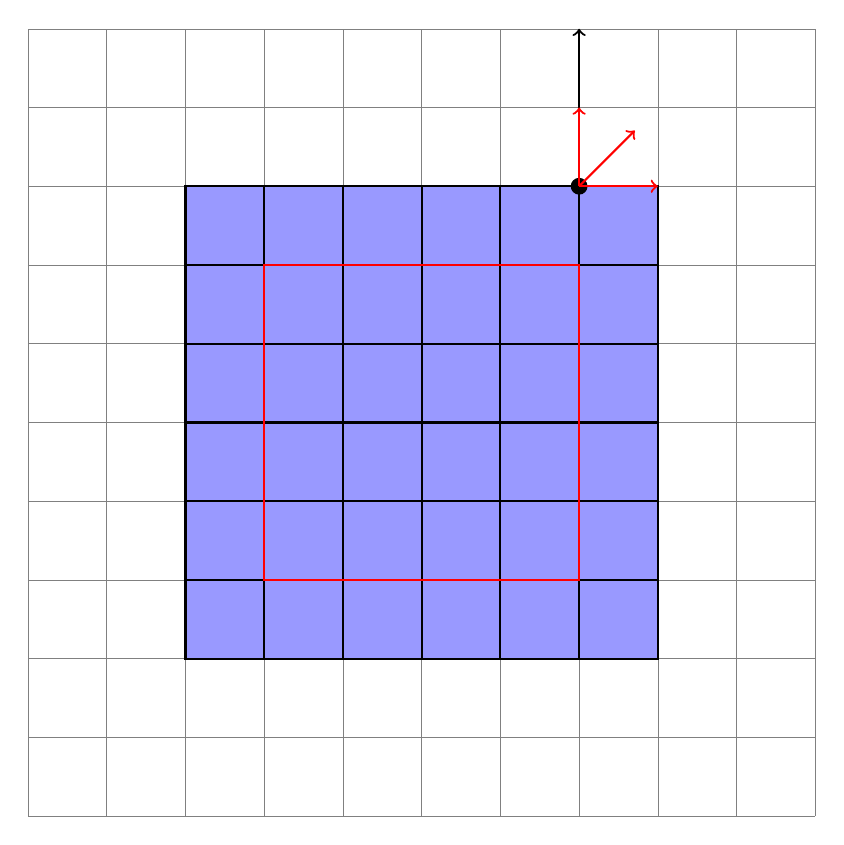
\begin{tikzpicture}
        % сетка
        \draw[step=1,gray,very thin] (-5,-5) grid (5,5);
        % тело
        \filldraw[fill=blue!40!white, draw=black,thick](0,0) rectangle (1,1);
        \filldraw[fill=blue!40!white, draw=black,thick](1,0) rectangle (2,1);
        \filldraw[fill=blue!40!white, draw=black,thick](0,1) rectangle (1,2);
        \filldraw[fill=blue!40!white, draw=black,thick](1,1) rectangle (2,2);
        \filldraw[fill=blue!40!white, draw=black,thick](0,2) rectangle (1,3);
        \filldraw[fill=blue!40!white, draw=black,thick](1,2) rectangle (2,3);
        \filldraw[fill=blue!40!white, draw=black,thick](2,2) rectangle (3,3);
        \filldraw[fill=blue!40!white, draw=black,thick](2,1) rectangle (3,2);
        \filldraw[fill=blue!40!white, draw=black,thick](2,0) rectangle (3,1);

        \filldraw[fill=blue!40!white, draw=black,thick](-0,0) rectangle (-1,1);
        \filldraw[fill=blue!40!white, draw=black,thick](-1,0) rectangle (-2,1);
        \filldraw[fill=blue!40!white, draw=black,thick](-0,1) rectangle (-1,2);
        \filldraw[fill=blue!40!white, draw=black,thick](-1,1) rectangle (-2,2);
        \filldraw[fill=blue!40!white, draw=black,thick](-0,2) rectangle (-1,3);
        \filldraw[fill=blue!40!white, draw=black,thick](-1,2) rectangle (-2,3);
        \filldraw[fill=blue!40!white, draw=black,thick](-2,2) rectangle (-3,3);
        \filldraw[fill=blue!40!white, draw=black,thick](-2,1) rectangle (-3,2);
        \filldraw[fill=blue!40!white, draw=black,thick](-2,0) rectangle (-3,1);

        \filldraw[fill=blue!40!white, draw=black,thick](0,-0) rectangle (1,-1);
        \filldraw[fill=blue!40!white, draw=black,thick](1,-0) rectangle (2,-1);
        \filldraw[fill=blue!40!white, draw=black,thick](0,-1) rectangle (1,-2);
        \filldraw[fill=blue!40!white, draw=black,thick](1,-1) rectangle (2,-2);
        \filldraw[fill=blue!40!white, draw=black,thick](0,-2) rectangle (1,-3);
        \filldraw[fill=blue!40!white, draw=black,thick](1,-2) rectangle (2,-3);
        \filldraw[fill=blue!40!white, draw=black,thick](2,-2) rectangle (3,-3);
        \filldraw[fill=blue!40!white, draw=black,thick](2,-1) rectangle (3,-2);
        \filldraw[fill=blue!40!white, draw=black,thick](2,-0) rectangle (3,-1);

        \filldraw[fill=blue!40!white, draw=black,thick](-0,-0) rectangle (-1,-1);
        \filldraw[fill=blue!40!white, draw=black,thick](-1,-0) rectangle (-2,-1);
        \filldraw[fill=blue!40!white, draw=black,thick](-0,-1) rectangle (-1,-2);
        \filldraw[fill=blue!40!white, draw=black,thick](-1,-1) rectangle (-2,-2);
        \filldraw[fill=blue!40!white, draw=black,thick](-0,-2) rectangle (-1,-3);
        \filldraw[fill=blue!40!white, draw=black,thick](-1,-2) rectangle (-2,-3);
        \filldraw[fill=blue!40!white, draw=black,thick](-2,-2) rectangle (-3,-3);
        \filldraw[fill=blue!40!white, draw=black,thick](-2,-1) rectangle (-3,-2);
        \filldraw[fill=blue!40!white, draw=black,thick](-2,-0) rectangle (-3,-1);
        
        
        \draw[red,thick](-2,-2) rectangle (2,2);
        
        \node[draw,circle,inner sep=2pt,fill] at (2,3) {};

        \draw[black,thick,->] (2,3) -- ++ (90:2);
        \draw[red,thick,->] (2,3) -- ++ (90:1);
        \draw[red,thick,->] (2,3) -- ++ (0:1);
        \draw[red,thick,->] (2,3) -- ++ (45:1);
    \end{tikzpicture}
\end{document}
